\newpage

\chapter{Chapter}

\section{Section}

\subsection{Subsection}

\subsubsection{Subsubsection}
My text here with \textbf{italics}, with \textbf{bold}, and a \href{https://davibarreira.github.io/}{link}.  Adding some math expression here with  $x=10$ and 
\begin{displaymath}
	d(\omega(t_0),\omega(t_1)) \leq \int^{t_1}_{t_0}g(s) ds.
\end{displaymath}
 Adding some code like  \lstinline[style=julia]{plots}. Note that the  \lstinline[style=julia]{using plots}  
\begin{lstlisting}[language=JuliaLocal, style=julia]
using PlutoUI
\end{lstlisting}

\begin{lstlisting}[language=JuliaLocal, style=julia]
begin
	using Plots
	y(x) = sin(x)
	Plots.plot(y,
		color=:blue)
end
\end{lstlisting}

\begin{figure}[H]
	\centering
	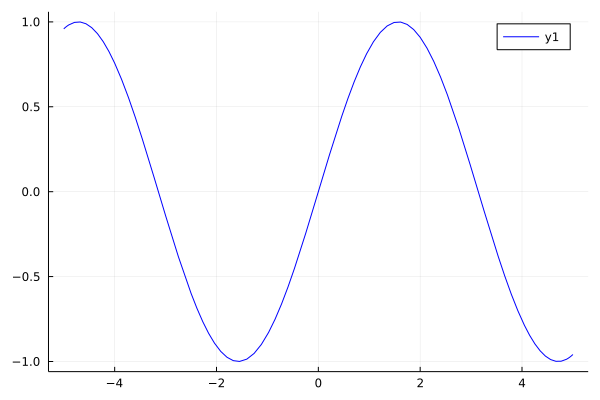
\includegraphics[width=0.8\textwidth]{./figures/notebooktest_figure1.png}
	\label{fig:notebooktest_figure1.png}

\end{figure}

\begin{lstlisting}[language=JuliaLocal, style=julia]
A = [10,10,10]
\end{lstlisting}

\begin{verbatim}
3-element Vector{Int64}:
 10
 10
 10
\end{verbatim}

\begin{lstlisting}[language=JuliaLocal, style=julia]
x = rand(10);
\end{lstlisting}

\begin{lstlisting}[language=JuliaLocal, style=julia]
x .+ 1
\end{lstlisting}

\begin{verbatim}
10-element Vector{Float64}:
 1.0043829775131798
 1.0776787708687692
 1.867001796168777
 1.7312374004771476
 1.2946190445975525
 1.816972735631969
 1.9086203975694922
 1.0381484595625103
 1.633243725670846
 1.2032637770963772
\end{verbatim}

\begin{lstlisting}[language=JuliaLocal, style=julia]
set_theme!(theme_ggplot2())
\end{lstlisting}

\begin{lstlisting}[language=JuliaLocal, style=julia]
Makie.plot(x)
\end{lstlisting}

\begin{figure}[H]
	\centering
	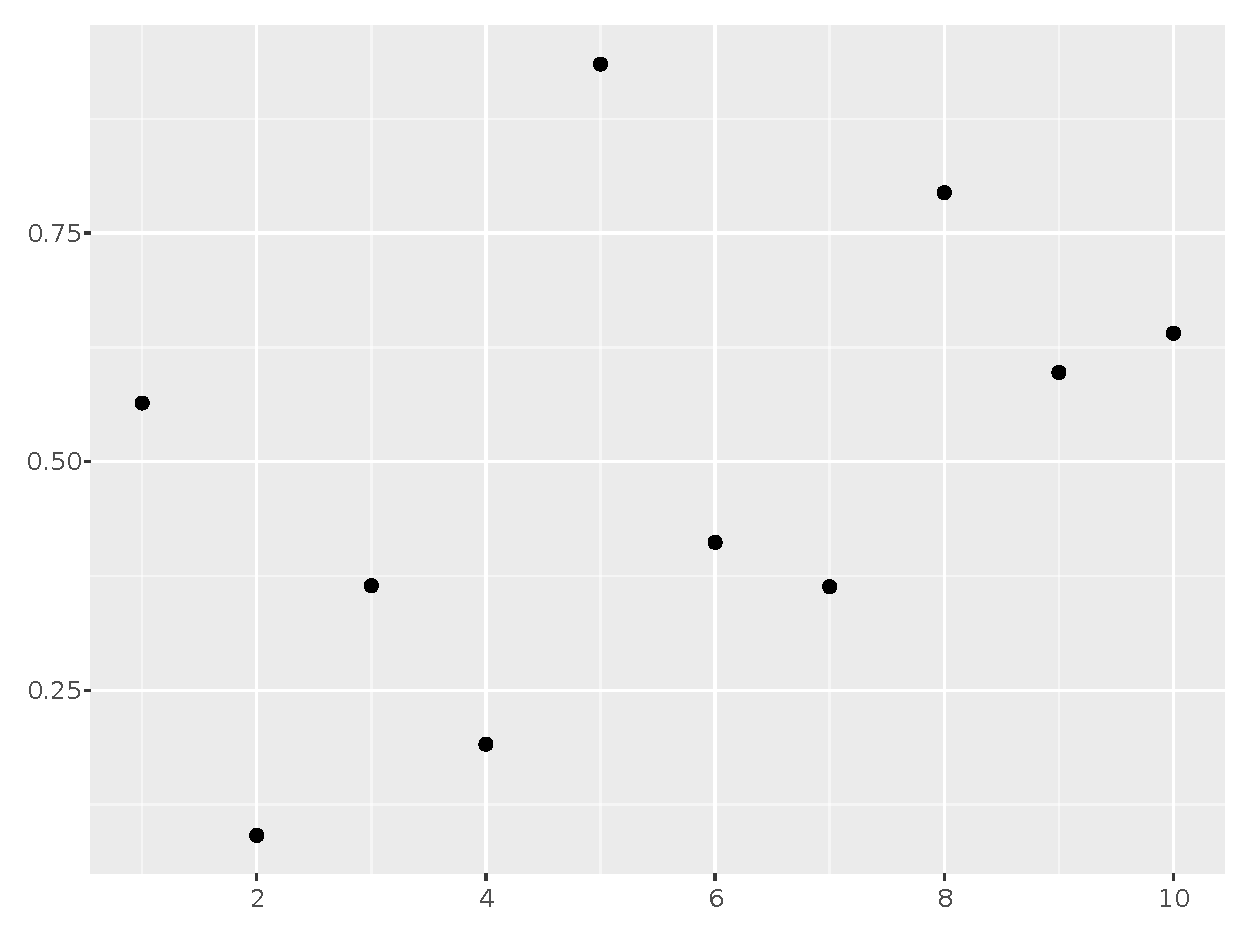
\includegraphics[width=0.8\textwidth]{./figures/notebooktest_figure2.pdf}
	\label{fig:notebooktest_figure2.pdf}

\end{figure}

\begin{lstlisting}[language=JuliaLocal, style=julia]
# PlutoUI.LocalResource("./figure.svg")
\end{lstlisting}

\begin{lstlisting}[language=JuliaLocal, style=julia]
# PlutoUI.LocalResource(figurepath)
\end{lstlisting}
